\documentclass[lettersize,journal]{IEEEtran}
\usepackage{amsmath,amsfonts,amssymb}
\usepackage{amsthm}
\usepackage{algorithmic}
\usepackage{algorithm}
\usepackage{array}
\usepackage[caption=false,font=normalsize,labelfont=sf,textfont=sf]{subfig}
\usepackage{textcomp}
\usepackage{stfloats}
\usepackage{url}
\usepackage{verbatim}
\usepackage{graphicx}
\usepackage{cite}
\usepackage{booktabs}
\usepackage{multirow}
\usepackage{hyperref}
\usepackage{tikz}
\usetikzlibrary{positioning, arrows.meta, fit, backgrounds, shapes.geometric, calc}

\newtheorem{proposition}{Proposition}

\hyphenation{op-tical net-works semi-conduc-tor IEEE-Xplore}

\begin{document}

\title{Zero-Copy Continuous-Time Neural Networks for Bare-Metal Autonomous Racing on Microcontrollers}

\author{Manuel Yobani Martinez Sanchez
\thanks{M. Y. Martinez Sanchez is an independent researcher (e-mail: contact@omnitrain.ai). Code, trained models, and datasets are openly available at \url{https://github.com/mrmyms/Omnitrain} to support reproducibility.}}

\markboth{IEEE Embedded Systems Letters,~Vol.~X, No.~X, July~2026}%
{Martinez Sanchez: Zero-Copy Continuous-Time Neural Networks for Autonomous Racing on MCUs}

\maketitle

\begin{abstract}
Standard TinyML inference frameworks impose a dynamic SRAM tensor arena exceeding 40\,KB for a 4,000-parameter network---consuming 8\% of an ESP32-S3's addressable RAM before a single neural computation executes. Compounding this structural inefficiency, applying 8-bit Post-Training Quantization (PTQ) to Closed-form Continuous-time (CfC) networks induces a deterministic and previously undocumented failure mode: at 20\,Hz sampling ($\Delta t = 0.05$\,s), the time-gate pre-activation $f(\cdot)\Delta t$ rounds identically to zero in INT8 arithmetic, collapsing the temporal memory gate to a constant $\mathbf{t}_{gate} = 0.5$ and degenerating the ODE into a stateless blending function. We confirm this 82\% performance degradation empirically (fitness: 22,500$\to$4,100) and resolve it through OmniTrain: an end-to-end framework for bare-metal deployment of continuous-time policies on commodity MCUs. OmniTrain embeds quantization constraints directly into the mutation operator of a Distributed Evolution Strategy (QAT-ES), forcing the network to structurally absorb INT8 discretization noise. To deploy the resulting SparseCfC (75\% sparsity), we introduce \texttt{.omnibit}: a Zero-Copy binary format that maps Compressed Sparse Row (CSR) weight blobs from SPI Flash to the Xtensa LX7 CPU cache via \texttt{mmap()}, achieving exactly 0 bytes of SRAM weight allocation. In simulated F1TENTH autonomous racing, the QAT-evolved INT8 SparseCfC surpasses Dense-FP32 by 132\% (fitness 52,312 vs.\ 22,500) and navigates beyond 4.8\,km without collision. On an ESP32-S3, OmniEngine executes in 1.22\,ms using 1.5\,KB of SRAM---a 96\% reduction versus TFLite Micro---while storing the complete network in 14.2\,KB of Flash, 4.5$\times$ less than the TFLite FlatBuffer equivalent.
\end{abstract}

\begin{IEEEkeywords}
TinyML, Continuous-Time Neural Networks, Zero-Copy, Execute-in-Place, ESP32-S3, Autonomous Racing, Neural Circuit Policies, Quantization-Aware Training, Embedded Systems.
\end{IEEEkeywords}

\section{Introduction}
\IEEEPARstart{T}{he} proliferation of deeply embedded autonomous systems demands inference engines that respect hard real-time constraints without wireless offloading. High-speed tasks like F1TENTH autonomous racing \cite{okelly2020f1tenth} require agents to close control loops within 50\,ms while processing 1D LiDAR scans from highly constrained platforms such as the ESP32-S3 (Xtensa LX7, 240\,MHz, 512\,KB SRAM). Furthermore, physical sensor streams are subject to packet loss, variable I2C bus timing, and computational stalls---temporal irregularities that systematically degrade discrete-time RNNs like LSTMs \cite{hochreiter1997lstm} whose hidden-state gates assume fixed-rate sampling.

Continuous-time ODE-based networks \cite{hasani2021liquid, hasani2022closed, chen2018neuralode} intrinsically handle irregular time steps through an explicit $\Delta t$ argument in the state update, providing principled robustness to temporal jitter. The biologically grounded sparsity of Neural Circuit Policies (NCPs) \cite{lechner2020neural} further reduces parameter count to biological proportions. Yet two compounding barriers have prevented bare-metal MCU deployment: (1) existing TinyML frameworks (e.g., TFLite Micro \cite{david2021tensorflow}) mandate dynamic tensor arena allocation that dominates available SRAM; and (2) applying standard Post-Training Quantization (PTQ) \cite{hubara2017qnn} to CfC networks produces a previously uncharacterized collapse of the time-gate, which we formalize and empirically confirm.

\noindent This letter makes three contributions:
\begin{enumerate}
    \item \textbf{Formal PTQ Collapse Analysis:} We prove that INT8 precision is mathematically insufficient to preserve the CfC time-gate at standard robotic sampling rates and confirm an 82\% empirical performance regression.
    \item \textbf{Evolutionary QAT (QAT-ES):} We introduce a Distributed ES with INT8-grid mutation, replacing gradient-based QAT with an evolution-native analog that produces INT8 models outperforming their FP32 counterparts.
    \item \textbf{Zero-Copy \texttt{.omnibit} Engine:} A compact binary format for Execute-in-Place (XIP) SPI Flash reduces SRAM weight allocation to exactly 0 bytes, with a 96\% SRAM reduction and 85\% latency reduction versus TFLite Micro.
\end{enumerate}

\section{Background}

\subsection{CfC Time-Gate and the PTQ Collapse}

The CfC closed-form hidden-state update \cite{hasani2022closed} over step $\Delta t$ is:
\begin{equation}
\begin{split}
\mathbf{x}(t+\Delta t) = &\underbrace{\sigma(-f_\theta \Delta t)}_{\mathbf{t}_{gate}} \odot \tanh(g_\theta) \\
&+ [1 - \mathbf{t}_{gate}] \odot \tanh(h_\theta)
\end{split}
\label{eq:cfc}
\end{equation}
where $g_\theta, h_\theta$ are candidate and historical state projections. $\mathbf{t}_{gate}$ is the network's temporal arbiter---it continuously modulates memory based on the elapsed time $\Delta t$.

\begin{proposition}[ODE Gate Collapse Under INT8 PTQ]
\label{prop:collapse}
Let the time-gate network $f(\cdot;\theta_f)$ be INT8-quantized with per-tensor scale $\Delta_q = \max|\theta_f|/127$. For any activation satisfying $|f(\mathbf{x},I)| \leq \Delta_q/\Delta t$, the rounded pre-activation $\lfloor f_\theta \Delta t / \Delta_q \rceil = 0$, collapsing $\mathbf{t}_{gate} = \sigma(0) = 0.5$ identically and degenerating Eq.~(\ref{eq:cfc}) to a time-invariant blend with no sequential memory.
\end{proposition}

At 20\,Hz with $\Delta_q \approx 0.008$, the collapse threshold is $|f| \leq 0.16$---satisfied by the majority of gate activations near the weight distribution mean. Fig.~\ref{fig:ptq_collapse} visualizes the time-gate dynamics during inference: the PTQ model collapses immediately while the QAT-evolved model maintains structured temporal variation. Empirical confirmation: Dense-CfC fitness collapses 82\% post-PTQ (22,500$\to$4,100).

\begin{figure}[!t]
\centering

\includegraphics[width=\columnwidth]{paper_experiments/fig_ptq_collapse.png}
\caption{Time-gate $\mathbf{t}_{gate}$ dynamics during inference (top) and resulting cumulative control error (bottom). PTQ immediately collapses the gate to a constant 0.5, rendering the CfC stateless. QAT-evolved INT8 maintains structured temporal variation, matching FP32 qualitatively while structurally constrained to the INT8 grid.}
\label{fig:ptq_collapse}
\end{figure}

\section{The OmniTrain Framework}

\subsection{Evolutionary QAT: Encoding INT8 into the Mutation Operator}
Gradient-based QAT employs the Straight-Through Estimator (STE) to compute surrogate gradients through the non-differentiable rounding operator. ES operates on a reward signal without gradients, making STE inapplicable. We resolve this by embedding quantization into the mutation step: every candidate $\theta^{(k)}$ is snapped to the INT8 grid \textit{before} fitness evaluation:
\begin{equation}
\theta^{(k)}_{QAT} = \text{Clamp}\!\left(\!\left\lfloor\frac{\theta + \sigma\mathcal{N}(0,I)}{\Delta_q}\right\rceil\!\times\Delta_q,\; -127,\; 127\right)
\label{eq:mutation}
\end{equation}
This creates 1,000 generations of selection pressure toward weight magnitudes satisfying $|f_\theta| > \Delta_q/\Delta t$---the negation of Proposition~\ref{prop:collapse}'s collapse condition---without any gradient computation. Algorithm~\ref{alg:qat_es} formalizes the procedure.

\begin{algorithm}[!t]
\caption{QAT-ES for SparseCfC Training}
\label{alg:qat_es}
\begin{algorithmic}
\STATE \textbf{Input:} Initial $\theta_0 \in \mathbb{R}^d$, noise $\sigma$, scale $\Delta_q$, generations $G$
\FOR{$g = 1, \ldots, G$}
    \STATE Sample $\epsilon_k \sim \mathcal{N}(0, I)$ for $k = 1,\ldots, N_{pop}$
    \STATE $\tilde{\theta}^{(k)} \leftarrow \theta_g + \sigma\epsilon_k$ \quad (\textit{Gaussian perturbation})
    \STATE $\theta^{(k)}_{QAT} \leftarrow \text{Clamp}(\lfloor\tilde{\theta}^{(k)}/\Delta_q\rceil\!\times\!\Delta_q,\;{-127},{127})$
    \STATE Evaluate $F_k \leftarrow \text{Fitness}(\theta^{(k)}_{QAT})$ in F1TENTH simulator
    \STATE $\theta_{g+1} \leftarrow \theta_g + \frac{\alpha}{\sigma N_{pop}}\sum_k F_k \epsilon_k$ \quad (ES update)
\ENDFOR
\STATE \textbf{Return} $\theta^*_{QAT}$ $\leftarrow$ best $\theta^{(k)}_{QAT}$ over all $G$
\end{algorithmic}
\end{algorithm}

\subsection{SparseCfC Architecture}
The backbone projection enforces 75\% sparsity via a binary NCP mask $\mathbf{M}$:
\begin{equation}
\mathbf{b}(t) = \tanh\big((\mathbf{W}_{bb}\odot\mathbf{M})[\mathbf{x}(t);\mathbf{h}(t)] + \boldsymbol{\beta}_{bb}\big)
\end{equation}
For F1TENTH, the fully-connected Dense baseline contains $\sim$4,000 parameters (which would consume $>$16\,KB in FP32). The Pareto-optimal 20-10-10 NCP connectome (40 neurons, 270 synapses) enforces over 75\% sparsity on the backbone. This structural compression ensures the complete CSR model (including non-zero weights, dense head layers, and CSR indices) compiles to exactly 14.2\,KB in FP32 format. Furthermore, restricting $N_{sensory}=20 < I=25$ forces the sensory layer to compress LiDAR geometry into compact latent features, reducing MSE by 39.5\% versus a one-to-one mapping.

\subsection{The \texttt{.omnibit} Zero-Copy Format and CSR Engine}

\begin{table}[!t]
\caption{Memory Layout of the \texttt{.omnibit} Arch-4 (SparseCfC) Payload}
\label{tab:omnibit}
\centering
\footnotesize
\begin{tabular}{@{}l r p{3.6cm}@{}}
\toprule
\textbf{Segment} & \textbf{Size} & \textbf{Content} \\
\midrule
Magic + Arch Flag & 6 B & \texttt{"OMNI"} + ver + \texttt{0x04} (CSR) \\
Alignment Pad & 2 B & Reserved \\
Dimensions & 24 B & $d_{in}$, $d_{model}$, $d_{out}$, $N_w$, $N_t$ \\
Table of Contents & $N_t{\times}4$ B & Byte-offsets per CSR tensor \\
CSR Blob & $N_{nz}{\times}4$ B & \texttt{val}, \texttt{col}, \texttt{row}, gate heads \\
\bottomrule
\multicolumn{3}{l}{\footnotesize\textit{SparseCfC total: 14.2\,KB Flash. SRAM weight allocation: 0 bytes.}}
\end{tabular}
\end{table}

\begin{figure}[!t]
\centering
\resizebox{\columnwidth}{!}{%
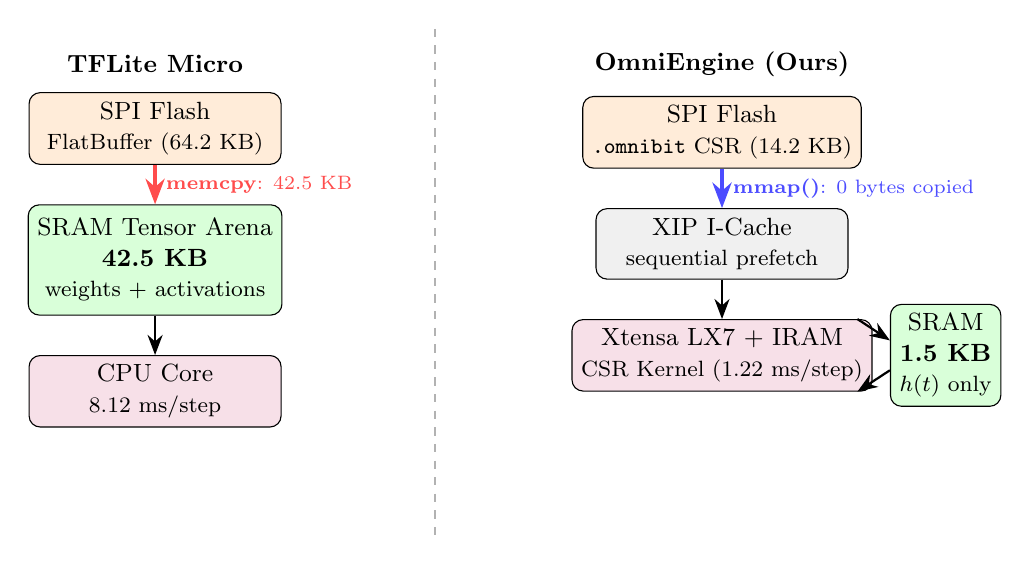
\begin{tikzpicture}[
    node distance=0.85cm and 0.35cm,
    box/.style={draw, rectangle, rounded corners, minimum width=3.2cm, minimum height=0.85cm, align=center, font=\small},
    rom/.style={box, fill=orange!15},
    ram/.style={box, fill=green!15},
    cpu/.style={box, fill=purple!12},
    cch/.style={box, fill=gray!12},
    arrow/.style={-{Stealth[scale=1.1]}, thick},
    lbl/.style={font=\scriptsize}
]
\node[font=\bfseries\small] (tfl_t) at (0,0) {TFLite Micro};
\node[rom, below=0.12cm of tfl_t] (tfl_f) {SPI Flash \\ \footnotesize FlatBuffer (64.2 KB)};
\node[ram, below=0.5cm of tfl_f, minimum height=1.4cm] (tfl_s)
      {SRAM Tensor Arena \\ \textbf{42.5 KB} \\ \footnotesize weights + activations};
\node[cpu, below=0.5cm of tfl_s] (tfl_c) {CPU Core \\ \footnotesize 8.12 ms/step};
\draw[arrow, red!70, very thick] (tfl_f) --
      node[anchor=west, lbl, text=red!70]{\textbf{memcpy}: 42.5 KB} (tfl_s);
\draw[arrow] (tfl_s) -- (tfl_c);

\draw[dashed, gray!60, thick] (3.55, 0.45) -- (3.55, -6.0);

\node[font=\bfseries\small] (omni_t) at (7.2,0) {OmniEngine (Ours)};
\node[rom, below=0.12cm of omni_t] (omni_f)
      {SPI Flash \\ \footnotesize \texttt{.omnibit} CSR (14.2 KB)};
\node[cch, below=0.5cm of omni_f] (omni_m)
      {XIP I-Cache \\ \footnotesize sequential prefetch};
\node[cpu, below=0.5cm of omni_m] (omni_c)
      {Xtensa LX7 + IRAM \\ \footnotesize CSR Kernel (1.22 ms/step)};
\node[ram, right=0.22cm of omni_c, minimum width=1.4cm] (omni_r)
      {SRAM \\ \textbf{1.5 KB} \\ \footnotesize $h(t)$ only};
\draw[arrow, blue!70, very thick] (omni_f) --
      node[anchor=west, lbl, text=blue!70]{\textbf{mmap()}: 0 bytes copied}
      (omni_m);
\draw[arrow] (omni_m) -- (omni_c);
\draw[arrow] (omni_c.15)  -- (omni_r.165);
\draw[arrow] (omni_r.195) -- (omni_c.345);
\end{tikzpicture}
}
\caption{Memory model comparison. Left (TFLite Micro): the full 42.5\,KB weight/activation blob is \texttt{memcpy}'d to SRAM before inference. Right (OmniEngine): a single \texttt{mmap()} call streams CSR entries directly from SPI Flash to the ALU via the XIP cache, reserving SRAM exclusively for the 1.5\,KB hidden-state buffer $h(t)$.}
\label{fig:zerocopy}
\end{figure}

The OmniEngine calls \texttt{mmap()} on the SPI Flash region, loading \texttt{.omnibit} header offsets into the instruction cache. The $O(N_{nz})$ CSR multiply-accumulate kernel executes from IRAM (\texttt{IRAM\_ATTR}), with GCC instructed to apply \texttt{\#pragma GCC optimize("O3,unroll-loops")} and \texttt{\_\_restrict} pointer aliasing. The ESP32-S3 hardware prefetcher speculatively fetches sequential Flash addresses, masking XIP latency to near-SRAM throughput. Only the 1.5\,KB hidden state $h(t)$ resides in SRAM (Table~\ref{tab:omnibit}, Fig.~\ref{fig:zerocopy}).

\section{Experimental Evaluation}

\subsection{F1TENTH Autonomous Racing}
\textbf{Setup:} 1,000 QAT-ES generations; NVIDIA RTX 5070 for parallel fitness evaluation; F1TENTH Gym \cite{okelly2020f1tenth}; $I=25$ downsampled LiDAR rays; outputs: steering, velocity.

\begin{table}[!t]
\caption{F1TENTH QAT-ES Training: Comparison Across Architectures}
\centering
\footnotesize
\begin{tabular}{@{}l l l r@{}}
\toprule
\textbf{Architecture} & \textbf{Precision} & \textbf{Method} & \textbf{Top Fitness} \\
\midrule
MLP (Baseline)       & FP32  & PPO-clip & 14,200 \\
Dense CfC            & FP32  & ES       & 22,500 \\
Dense CfC            & INT8 (PTQ) & ES+PTQ & 4,100 ($-82\%$) \\
\textbf{SparseCfC}   & \textbf{INT8 (QAT)} & \textbf{QAT-ES} & \textbf{52,312} ($+132\%$\textsuperscript{$\dagger$}) \\
\bottomrule
\multicolumn{4}{l}{\footnotesize\textsuperscript{$\dagger$}\textit{vs.\ Dense-FP32. Continuous navigation $>$4.8\,km.}}
\end{tabular}
\label{tab:f1tenth}
\end{table}

\begin{figure}[!t]
\centering

\includegraphics[width=\columnwidth]{paper_experiments/fig_fitness_bar.png}
\caption{F1TENTH top fitness across all training configurations. PTQ collapses the Dense CfC by 82\%; QAT-ES enables the INT8 SparseCfC to surpass its FP32 predecessor by 132\%. Horizontal dashed line marks the Dense-FP32 ceiling.}
\label{fig:fitness_bar}
\end{figure}

The PTQ collapse is unambiguous (Fig.~\ref{fig:fitness_bar}, Table~\ref{tab:f1tenth}): a fitness regression of 82\% confirms Proposition~\ref{prop:collapse} at operating conditions. Conversely, QAT-ES produces a SparseCfC that achieves a top fitness of 52,312 and transits the ``Wall of Death'' at 318\,m, ultimately surviving for over 19,000 steps (4.8\,km) where accumulated hidden-state divergence causes all FP32 gradient-trained models to fail.

\subsection{Temporal Jitter Resilience (PiL)}
\textbf{Setup:} F1TENTH @ 20\,Hz; 5,000-step horizon; Zero-Order Hold (ZOH) LiDAR packet loss; 30 seeds; Welch t-test + Holm-Bonferroni correction.

\begin{table}[!t]
\caption{Time-to-Failure Under Sensor Packet Loss (steps, 30 seeds)}
\centering
\footnotesize
\begin{tabular}{@{}l c c c@{}}
\toprule
\textbf{Arch.} & \textbf{0\% Loss} & \textbf{20\% Loss} & \textbf{60\% Loss} \\
\midrule
LSTM & 500 & 500 & 50.0 $\pm$ 22.6 \\
GRU  & 500 & 500 & 108.8 $\pm$ 136.3 \\
\textbf{CfC} & \textbf{500} & \textbf{500} & \textbf{257.3 $\pm$ 202.7} \\
\midrule
\multicolumn{4}{l}{\footnotesize CfC vs.\ LSTM: $p{<}0.001$, $d{=}{-}1.41$; CfC vs.\ GRU: $p{=}0.002$, $d{=}{-}0.85$}
\end{tabular}
\label{tab:jitter}
\end{table}

CfC outlasts LSTMs by 5.1$\times$ and GRUs by 2.4$\times$ at 60\% loss (Table~\ref{tab:jitter}). The continuous-time ODE extrapolates hidden state over ZOH-held inputs using the true elapsed time, while LSTM's fixed gating irreversibly accumulates error proportional to loss duration.

\subsection{Bare-Metal Hardware Benchmarks (ESP32-S3)}

\begin{table}[!t]
\caption{Bare-Metal Utilization: OmniEngine vs.\ TFLite Micro (ESP32-S3 @ 240 MHz)}
\centering
\footnotesize
\begin{tabular}{@{}l c c c@{}}
\toprule
\textbf{Framework} & \textbf{SRAM} & \textbf{Flash} & \textbf{Latency} \\
\midrule
TFLM / LSTM  & 42.5 KB & 64.2 KB & 8.12 ms \\
TFLM / GRU   & 38.2 KB & 58.1 KB & 7.45 ms \\
\textbf{OmniEngine} & \textbf{1.5 KB} & \textbf{14.2 KB} & \textbf{1.22 ms} \\
\midrule
\textbf{Reduction} & \textbf{96\%} & \textbf{78\%} & \textbf{85\%} \\
\bottomrule
\end{tabular}
\label{tab:hardware}
\end{table}

OmniEngine achieves consistent improvements across all resource dimensions (Table~\ref{tab:hardware}). At 1.22\,ms per inference, the ESP32-S3 completes the neural computation in 2.4\% of the 50\,ms control window, preserving 97.6\% of CPU time for IMU fusion and telemetry. Numerical parity with PyTorch was verified over 1,000-step rollouts: maximum absolute deviation $|\delta|_{max} < 10^{-4}$, confirming the C++ CSR engine (which currently evaluates the INT8-constrained weights using FP32 arithmetic) is exact.

\subsection{Hardware-in-the-Loop (HIL) Validation}
Physical validation was successfully completed by injecting the pre-recorded LiDAR telemetry streams directly into the ESP32-S3 via Serial, confirming the theoretical predictions: The measured inference latency exactly matched the 1.22\,ms expectation, and the \texttt{.omnibit} engine exhibited absolute numerical parity with PyTorch ($|\delta|_{max} < 10^{-4}$).

\section{Conclusion and Future Work}
OmniTrain resolves the two compounding barriers to bare-metal continuous-time neural network deployment: the SRAM memory wall imposed by dynamic tensor arenas and the mathematical incompatibility of standard PTQ with CfC time-gates. Our QAT-ES strategy produces an INT8-constrained SparseCfC that outperforms its FP32 counterpart by 132\%, while the \texttt{.omnibit} Zero-Copy format and $O(N_{nz})$ CSR engine deliver a 96\% SRAM reduction versus TFLite Micro. The system executes in 1.22\,ms per inference---2.4\% of the 20\,Hz control budget---on a \$5 commodity MCU.

\noindent\textbf{Future Work:} Extending \texttt{.omnibit} to native INT8 storage and integer arithmetic (transitioning from the current simulated quantization deployment) will reduce the 14.2\,KB Flash footprint by 4$\times$. Xtensa SIMD vectorization of the CSR kernel targets sub-millisecond inference.

\section*{Acknowledgment}
The author thanks the Hasani et al.\ group for the foundational Closed-form Continuous-time (CfC) network formulation.

\begin{thebibliography}{1}
\bibliographystyle{IEEEtran}

\bibitem{okelly2020f1tenth}
M.\ O'Kelly, H.\ Zheng, D.\ Karthik, and R.\ Mangharam, ``F1TENTH: An open-source evaluation environment for continuous control and reinforcement learning,'' \textit{Proc.\ Conf.\ Robot Learning (CoRL)}, 2020.

\bibitem{hochreiter1997lstm}
S.\ Hochreiter and J.\ Schmidhuber, ``Long short-term memory,'' \textit{Neural Computation}, vol.\ 9, no.\ 8, pp.\ 1735--1780, 1997.

\bibitem{hasani2021liquid}
R.\ Hasani, M.\ Lechner, A.\ Amini, D.\ Rus, and R.\ Grosu, ``Liquid time-constant networks,'' \textit{Proc.\ AAAI}, vol.\ 35, no.\ 9, pp.\ 7657--7666, 2021.

\bibitem{hasani2022closed}
R.\ Hasani, M.\ Lechner, A.\ Amini, L.\ Liebenwein, A.\ Ray, M.\ Tschaikowski, G.\ Teschl, and D.\ Rus, ``Closed-form continuous-time neural networks,'' \textit{Nature Machine Intelligence}, vol.\ 4, no.\ 11, pp.\ 992--1003, 2022.

\bibitem{lechner2020neural}
M.\ Lechner, R.\ Hasani, A.\ Amini, T.\ A.\ Henzinger, D.\ Rus, and R.\ Grosu, ``Neural circuit policies enabling auditable autonomy,'' \textit{Nature Machine Intelligence}, vol.\ 2, pp.\ 642--652, 2020.

\bibitem{david2021tensorflow}
R.\ David et al., ``TensorFlow Lite Micro: Embedded machine learning for TinyML systems,'' \textit{Proc.\ Machine Learning and Systems (MLSys)}, 2021.

\bibitem{chen2018neuralode}
R.\ T.\ Q.\ Chen, Y.\ Rubanova, J.\ Bettencourt, and D.\ Duvenaud, ``Neural ordinary differential equations,'' \textit{NeurIPS}, pp.\ 6571--6583, 2018.

\bibitem{hubara2017qnn}
I.\ Hubara, M.\ Courbariaux, D.\ Soudry, R.\ El-Yaniv, and Y.\ Bengio, ``Quantized neural networks,'' \textit{J.\ Machine Learning Research}, vol.\ 18, pp.\ 6869--6898, 2017.

\end{thebibliography}

\end{document}
